% Generated by book/tools/notebook_to_tex.py. Do not edit by hand.

\chapter[KoGPT2 SFT (Instruction Tuning)]{KoGPT2 SFT (Instruction Tuning)}

\label{ch:28}

\markboth{KoGPT2 SFT (Instruction Tuning)}{KoGPT2 SFT (Instruction Tuning)}

\chaptermeta{28_sft/28_sft.ipynb}{https://colab.research.google.com/github/yoon-gu/neuqes-101/blob/master/28_sft/28_sft.ipynb}{KoGPT2를 KoAlpaca instruction-response 데이터로 SFT해 지시를 따르는 행동 정렬을 확인}



\index{1KoGPT2@KoGPT2}

\index{1SFT@SFT}

\index{1Instruction Tuning@Instruction Tuning}

\index{1Supervised Fine Tuning@Supervised Fine-Tuning}

\index{1behavior alignment@behavior alignment}

\index{1KoAlpaca@KoAlpaca}

\index{1beomi KoAlpaca v1 1a@beomi/KoAlpaca-v1.1a}

\index{1trl@trl}

\index{1SFTTrainer@SFTTrainer}

\index{1SFTConfig@SFTConfig}

\index{1completion only loss True@completion\_only\_loss=True}

\index{1completion mask@completion\_mask}

\index{1labels 100@labels=-100}

\index{1response only loss@response-only loss}

\index{1prompt masking@prompt masking}

\index{1PreTrainedTokenizerFast@PreTrainedTokenizerFast}

\index{1AutoModelForCausalLM@AutoModelForCausalLM}

\index{1CrossEntropyLoss@CrossEntropyLoss}

\index{0지시 튜닝@지시 튜닝}

\index{0지도 미세조정@지도 미세조정}

\index{0행동 정렬@행동 정렬}

\index{0응답 구간 손실@응답 구간 손실}

\index{0프롬프트 마스킹@프롬프트 마스킹}

\index{0답변 토큰@답변 토큰}

\index{1instruction following@instruction following}

\index{1DataCollatorForCompletionOnlyLM removed@DataCollatorForCompletionOnlyLM removed}

\index{1TRL 1 5 1@TRL 1.5.1}

\index{1SFTConfig completion only loss True@SFTConfig(completion\_only\_loss=True)}

\index{1prompt column@prompt column}

\index{1completion column@completion column}

\index{1completion mask@completion mask}

\index{1prompt tokens masked@prompt tokens masked}

\index{1answer tokens learned@answer tokens learned}

\index{1labels 100 thread@labels=-100 thread}

\index{1MLM vs CausalLM vs SFT@MLM vs CausalLM vs SFT}

\index{1fine tuning meaning shift@fine-tuning meaning shift}

\index{1task head vs behavior alignment@task head vs behavior alignment}

\index{1response template@response template}

\index{1chat template@chat template}

\index{1KoGPT2 SFT@KoGPT2 SFT}

\index{1KoAlpaca SFT@KoAlpaca SFT}

\index{0응답 마스킹@응답 마스킹}

\index{0지시 따르기@지시 따르기}

\index{0파인튜닝 의미 변화@파인튜닝 의미 변화}

\index{0프롬프트 제외@프롬프트 제외}

\index{0답변만 학습@답변만 학습}

\index{1completion only loss@completion\_only\_loss}



\section{누적 추적표}

\begin{booktable}{28장 누적 추적표 표}{tab:ch28-01}
\begin{adjustbox}{max width=\textwidth}
\begin{tabular}{@{}llllll@{}}
\toprule
Ch & 모델 & 토크나이저 & 데이터 & \inlinecode{labels\ =\ -100} 자리 & Loss \\
\midrule

25 & \inlinecode{gpt2} (124M, 사전학습) & BPE (gpt2 그대로, vocab 50,257) & 영어 TinyStories 30K & pad 만 & \inlinecode{CrossEntropyLoss} (next-token) - continual pretraining \\
26 & 작은 GPT2 (한국어, 약 3M, scratch) & BBPE (직접 학습, vocab 약 4,000) & 한국어 TinyStories 30K & pad 만 & \inlinecode{CrossEntropyLoss} (next-token) \\
27 & KoGPT2 \inlinecode{skt/kogpt2-base-v2} (125M) & BBPE (KoGPT2 그대로, vocab 51,200) & 한국어 TinyStories 30K & pad 만 & \inlinecode{CrossEntropyLoss} (next-token) - continual pretraining \\
\textbf{28 \(\leftarrow\) 여기} & \textbf{KoGPT2 \inlinecode{skt/kogpt2-base-v2} (125M, 동일)} & \textbf{BBPE (KoGPT2 그대로, vocab 51,200, 동일)} & \textbf{KoAlpaca instruction-response 쌍 (약 3K, 3,000 샘플)} & \textbf{prompt 부분 (\inlinecode{\#\#\#\ 응답:} 앞 전부)} & \textbf{\inlinecode{CrossEntropyLoss} (next-token, \emph{답변 부분만}) --- SFT} \\
29 (다음) & \ref{ch:28}장 SFT 모델 + 비교 & (동일) & 분야별 벤치마크 (KMMLU / HAERAE / MMLU ...) & - (평가만) & - (\inlinecode{lm-evaluation-harness}) \\
\bottomrule
\end{tabular}
\end{adjustbox}
\end{booktable}

전체 장 표는 \href{https://github.com/yoon-gu/neuqes-101\#챕터별-변화추적표}{루트 README} 를 참고하세요.

\begin{center}\rule{0.5\linewidth}{0.5pt}\end{center}

\section{GPT 시대 학습 4단계 --- 본 장의 위치 (단계 3, SFT)}

\ref{ch:24}장에서 도입한 GPT 시대 학습 4단계 표. 본 장은 \emph{단계 3 (SFT)} --- \emph{행동 정렬} 이 처음 일어나는 단계입니다.

\begin{booktable}{28장 GPT 시대 학습 4단계 - 본 장의 위치 (단계 3, SFT) 표}{tab:ch28-02}
\begin{adjustbox}{max width=\textwidth}
\begin{tabular}{@{}llllll@{}}
\toprule
단계 & 정확 용어 & 의미 & \inlinecode{labels\ =\ -100} 자리 & 본 커리큘럼 & 본 장? \\
\midrule

1 & \textbf{Pretraining} (사전학습) & random init 본체 + 일반 코퍼스 & pad 만 & \ref{ch:24}장 (영어), \ref{ch:26}장 (한국어) & \\
2 & \textbf{Continual pretraining} (계속 사전학습) & 사전학습된 본체 + 새 데이터, \emph{같은 CausalLM task} & pad 만 & \ref{ch:25}장 (영어), \ref{ch:27}장 (한국어) & \\
3 & \textbf{SFT} (Supervised Fine-Tuning / Instruction tuning) & instruction-response 쌍으로 \emph{행동 정렬}. \emph{답변 부분만} 학습 & \textbf{prompt 부분} & \textbf{\ref{ch:28}장 \(\leftarrow\) 여기} & OK \\
4 & \textbf{Alignment} (DPO / RLHF / GRPO) & preference 또는 verifier reward 로 \emph{선호 정렬} & (RL 내부, response 부분만) & \ref{ch:30}장 (DPO), \ref{ch:31}장 (GRPO) & \\
\bottomrule
\end{tabular}
\end{adjustbox}
\end{booktable}

\subsection{\texorpdfstring{단계 2 (\ref{ch:27}장) \(\to\) 단계 3 (\ref{ch:28}장) 의 결정적 변화}{단계 2 (\ref{ch:27}장) \textbackslash to 단계 3 (\ref{ch:28}장) 의 결정적 변화}}

\begin{itemize}
\tightlist
\item
  \textbf{단계 2 (continual pretraining)}: \emph{연속된 일반 텍스트} 를 \emph{거의 모든 자리} 에서 학습. 모델은 \emph{다음 토큰 분포} 를 도메인에 맞게 다듬을 뿐 --- \emph{지시를 따르는 법} 은 배우지 않음
\item
  \textbf{단계 3 (SFT)}: \emph{instruction-response 쌍} 에서 \emph{답변 토큰만} 학습. 모델은 \emph{주어진 지시에 어떻게 응답하는가} 를 배움 --- \textbf{행동 정렬 (behavior alignment)}
\end{itemize}

\begin{quote}
\emph{같은 본체, 같은 loss 종류, 단 데이터 형식 + 마스킹 자리만 바뀌어} 모델이 \emph{지시를 따라가게} 됩니다. 그 한 줄이 \texttt{labels{[}:prompt\_len{]}\ =\ -100}. 본 장은 그 한 줄을 \emph{눈으로 확인} 하는 장입니다.
\end{quote}



\section{변경점: \ref{ch:27}장 대비}

\begin{booktable}{28장 변경점 요약}{tab:ch28-03}
\begin{adjustbox}{max width=\textwidth}
\begin{tabular}{@{}lll@{}}
\toprule
축 & \ref{ch:27}장 (KoGPT2 continual pretraining) & \ref{ch:28}장 (본 장, KoGPT2 SFT) \\
\midrule

본체 & KoGPT2 \inlinecode{skt/kogpt2-base-v2} (125M) & \textbf{KoGPT2 \inlinecode{skt/kogpt2-base-v2} (125M, 동일)} \(\leftarrow\) 고정 \\
토크나이저 & \inlinecode{PreTrainedTokenizerFast} (KoGPT2 BBPE, vocab 51,200) & \textbf{(동일)} \(\leftarrow\) 고정 \\
Loss 종류 & next-token \inlinecode{CrossEntropyLoss} & \textbf{next-token \inlinecode{CrossEntropyLoss} (종류 동일)} \(\leftarrow\) 고정 \\
\textbf{데이터 형식} & 연속된 일반 텍스트 (TinyStories) & \textbf{instruction-response 쌍 (KoAlpaca)} \(\leftarrow\) \emph{변화 1} \\
\textbf{Trainer} & \inlinecode{transformers.Trainer} & \textbf{\inlinecode{trl.SFTTrainer}} \(\leftarrow\) \emph{변화 2} (새 클래스, 첫 등장) \\
\textbf{\inlinecode{labels\ =\ -100} 자리} & pad 만 (거의 모든 자리 학습) & \textbf{prompt 부분 전체 (\inlinecode{\#\#\#\ 응답:} 앞)} \(\leftarrow\) \emph{변화 3, 핵심} \\
효과 & 도메인 적응 (동화 풍) & \textbf{instruction 따라가기 (행동 정렬)} \(\leftarrow\) 메시지 \\
lr & 2e-5 & 2e-5 (SFT 표준, 동일 범위) \\
\bottomrule
\end{tabular}
\end{adjustbox}
\end{booktable}

\begin{quote}
\textbf{핵심}: \emph{본체·토크나이저·loss 종류는 그대로}. 바뀌는 건 \emph{데이터 형식 + trainer + 마스킹 자리} 세 가지. 그중에서도 \textbf{\inlinecode{labels} 마스킹 자리} 가 \emph{왜 모델이 instruction 을 따라가게 되는가} 의 진짜 원인입니다. \ref{ch:27}장의 collator 가 \emph{거의 모든 자리} 를 학습했다면, \ref{ch:28}장 은 \emph{prompt 를 전부 가리고 답변만} 학습합니다 --- \emph{정확히 정반대 자리}.
\end{quote}



\section{\texorpdfstring{\inlinecode{labels\ =\ -100} thread 의 완성 --- 세 단계를 한 화면에}{labels = -100 thread 의 완성 --- 세 단계를 한 화면에}}

커리큘럼 전체를 관통하는 thread 의 \emph{종착점} 입니다. \inlinecode{labels\ =\ -100} 은 \emph{그 자리를 loss 에서 제외} 하라는 의미 (\inlinecode{CrossEntropyLoss(ignore\_index=-100)}). \textbf{어느 자리를 -100 으로 두느냐가 곧 모델이 무엇을 학습하느냐} 를 결정합니다.

\begin{booktable}{28장 labels = -100 thread 의 완성 - 세 단계를 한 화면에 표}{tab:ch28-04}
\begin{adjustbox}{max width=\textwidth}
\begin{tabular}{@{}llllll@{}}
\toprule
단계 & 장 & task & \inlinecode{labels\ =\ -100} 자리 & loss 계산 자리 & 모델이 배우는 것 \\
\midrule

\textbf{MLM} & \ref{ch:20}·\ref{ch:21}장·22 & 양방향 빈칸 채우기 & 선택 안 된 약 85\% (= 안 가린 자리) & \textbf{선택된 약 15\% (가린 자리) 만} & 문맥으로 \emph{가려진 단어} 복원 \\
\textbf{CausalLM} & \ref{ch:24}·\ref{ch:25}장·26·27 & 다음 토큰 예측 & \textbf{pad 만} (거의 없음) & \textbf{거의 전 토큰} & \emph{다음에 올 토큰} 분포 \\
\textbf{SFT (본 장)} & \textbf{\ref{ch:28}장} & instruction 따라가기 & \textbf{prompt 부분 전체} (\inlinecode{\#\#\#\ 응답:} 앞) & \textbf{답변 토큰만} & \emph{지시에 대한 응답} 생성 \\
\bottomrule
\end{tabular}
\end{adjustbox}
\end{booktable}

\subsection{\texorpdfstring{세 단계를 한눈에 --- \emph{같은 \inlinecode{-100}, 다른 자리}}{세 단계를 한눈에 --- 같은 -100, 다른 자리}}

\Needspace{10\baselineskip}
\begin{lstlisting}
MLM (21장):     [the] [MASK] [sat] [on] [the] [MASK]
labels:          -100   cat   -100  -100 -100   mat       <- 가린 15% 만 학습

CausalLM (27장): [옛날] [옛날에] [작은] [소녀가] [살았어요]
labels:           옛날에  작은    소녀가  살았어요   <eos>      <- 거의 전부 학습 (shift)

SFT (28장):     [### 명령어:] [피보나치 설명] [### 응답:] [피보나치는] [수열입니다]
labels:           -100  -100   -100  -100  -100   -100   피보나치는  수열입니다   <- 답변만 학습
\end{lstlisting}

\begin{quote}
\textbf{MLM 은 일부 (15\%) 만 가리고}, \textbf{CausalLM 은 거의 안 가리고}, \textbf{SFT 는 prompt 전부 가립니다}. 세 task 모두 \emph{같은 \inlinecode{CrossEntropyLoss(ignore\_index=-100)}} 를 쓰지만 \emph{-100 의 자리} 가 다릅니다. \textbf{\ref{ch:28}장에서 이 thread 가 완성됩니다} --- 아래 §3 에서 KoGPT2 의 실제 collator 출력을 print 로 \emph{눈으로 확인} 합니다 (\ref{ch:21}장의 \texttt{{[}MASK{]}} 80/10/10 시각화의 SFT 판).
\end{quote}

핵심 메시지: \textbf{모델이 instruction 을 “따라간다” 는 것은, instruction 토큰 자체는 학습하지 않고 그에 대한 \emph{응답만} 학습한다는 의미}. 만약 prompt 도 함께 학습하면 모델은 \emph{질문 자체를 외우는} 쪽으로 기웁니다 --- 우리가 원하는 건 \emph{질문에 답하는 법} 입니다. 그 차이가 한 줄 \texttt{labels{[}:prompt\_len{]}\ =\ -100} 입니다.



\section{\texorpdfstring{“파인튜닝” 의미 변화의 완성 --- task head \(\to\) behavior alignment}{“파인튜닝” 의미 변화의 완성 --- task head \textbackslash to behavior alignment}}

커리큘럼 전체에서 \emph{fine-tune} 이라는 단어는 \emph{세 의미} 로 쓰였습니다. \ref{ch:28}장 이 그 세 번째 의미 (\emph{행동 정렬}) 의 도착점입니다.

\begin{booktable}{28장 “파인튜닝” 의미 변화의 완성 - task head \textbackslash to behavior alignment 표}{tab:ch28-05}
\begin{adjustbox}{max width=\textwidth}
\begin{tabular}{@{}llll@{}}
\toprule
의미 & 무엇이 바뀌나 & 장 & 비유 \\
\midrule

\textbf{1 task adaptation} (BERT 파인튜닝) & 본체 + \textbf{새 head} (\inlinecode{Linear(H,\ K)}) + \textbf{새 task loss} & \ref{ch:09}--\ref{ch:23}장 (분류) & \emph{새 도구} 를 손에 붙임 \\
\textbf{2 데이터 적응} (GPT continual pretraining) & head 그대로, \textbf{같은 next-token task}, \emph{새 데이터} & \ref{ch:25}·\ref{ch:27}장 & \emph{같은 도구} 로 \emph{새 재료} 연습 \\
\textbf{3 행동 정렬} (GPT SFT) & head 그대로, \textbf{같은 next-token CE}, \emph{instruction 형식 데이터} + \emph{prompt 마스킹} & \textbf{\ref{ch:28}장 \(\leftarrow\) 여기} & \emph{도구는 그대로}, \emph{지시를 따르는 법} 을 깨움 \\
\bottomrule
\end{tabular}
\end{adjustbox}
\end{booktable}

\subsection{\texorpdfstring{BERT 파인튜닝 (1) vs GPT SFT (3) --- \emph{진짜} instruction following}{BERT 파인튜닝 (1) vs GPT SFT (3) --- 진짜 instruction following}}

\begin{itemize}
\tightlist
\item
  \textbf{BERT 파인튜닝 (1)}: task 마다 \emph{다른 head} 를 붙입니다. 감정분류 head, NER head, QA head... \emph{task 하나당 모델 하나}. head 가 task 를 정의
\item
  \textbf{GPT SFT (3)}: \emph{head 는 LM head 하나 그대로}. \emph{입력 프롬프트 형식} 만 바꾸면 \emph{같은 모델} 이 번역도, 요약도, 질의응답도 합니다. \textbf{task 가 head 가 아니라 prompt 에 인코딩됨}
\end{itemize}

\begin{quote}
\emph{왜 GPT 하나가 모든 task 를 해내는가?} --- 답은 SFT 입니다. 본체는 \emph{입력 프롬프트만 바꾸면 다른 일} 을 하도록 \emph{행동 정렬} 되어 있습니다. \textbf{SFT 가 그 능력을 깨우는 단계}. BERT 가 \emph{task 마다 head 를 갈아끼우던} 시대에서, GPT 가 \emph{prompt 하나로 모든 task} 를 하는 시대로의 전환 --- 그 전환점이 본 장입니다.
\end{quote}

이게 \emph{진짜} behavior tuning 입니다 --- \emph{task 적응 (1)} 도, \emph{데이터 적응 (2)} 도 아닌, \emph{모델의 행동 자체} 를 instruction 을 따르도록 정렬하는 단계.



\section{\texorpdfstring{Loss --- next-token CE 동일, 단 \emph{어느 자리에서 계산하는가}}{Loss --- next-token CE 동일, 단 어느 자리에서 계산하는가}}

본 장의 loss 는 \ref{ch:27}장과 \emph{같은 종류} --- next-token \inlinecode{CrossEntropyLoss}:

\begin{equation}
\label{eq:ch28-01}
L_{\text{CLM}} = -\sum_{i} \log P(x_{i+1} \mid x_{\leq i})
\end{equation}

식~\eqref{eq:ch28-01}은 이 절에서 사용하는 핵심 관계를 정리한 것입니다.

다른 점은 \textbf{어느 위치 \(i\) 에서 합산하느냐} 입니다. SFT 는 \emph{답변 부분 토큰만} 합산합니다:

\begin{equation}
\label{eq:ch28-02}
L_{\text{SFT}} = -\sum_{i \in \text{response}} \log P(x_{i+1} \mid x_{\leq i}) \qquad (\text{prompt 부분은 } -100 \text{ 으로 제외})
\end{equation}

식~\eqref{eq:ch28-02}은 이 절에서 사용하는 핵심 관계를 정리한 것입니다.

\subsection{왜 prompt 도 학습하면 안 되나 --- 숫자로 감 잡기}

instruction \texttt{“\#\#\#\ 명령어:\textbackslash{}n2+2\ 는?\textbackslash{}n\textbackslash{}n\#\#\#\ 응답:\textbackslash{}n”} 뒤에 답변 \inlinecode{"4\ 입니다."} 가 오는 한 샘플을 생각해 봅시다. 토큰이 \emph{prompt 12개 + 답변 4개} 라고 하면:

\begin{booktable}{28장 왜 prompt 도 학습하면 안 되나 - 숫자로 감 잡기 표}{tab:ch28-06}
\begin{adjustbox}{max width=\textwidth}
\begin{tabular}{@{}lll@{}}
\toprule
학습 방식 & loss 합산 자리 & 모델이 강화하는 것 \\
\midrule

\textbf{전체 학습} (prompt 포함) & 16개 토큰 전부 & \emph{“\#\#\# 명령어:” \(\to\) “2+2 는?”} 같은 \emph{질문 자체의 패턴} 까지 외움 \\
\textbf{response-only} (본 장) & 답변 4개만 & \emph{prompt 가 주어졌을 때 답변} 하는 능력만 \\
\bottomrule
\end{tabular}
\end{adjustbox}
\end{booktable}

전체 학습을 하면 loss 의 \emph{대부분} 이 \emph{prompt 토큰} 에서 나옵니다 (prompt 가 보통 더 김). 그러면 모델은 \emph{질문을 받아쓰는 데} gradient 를 낭비합니다. 우리가 원하는 건 \emph{질문을 외우는 게 아니라 답하는 법} --- 그래서 prompt 를 \inlinecode{-100} 으로 가립니다.

\subsection{response-only 의 직관}

\begin{booktable}{28장 response-only 의 직관 표}{tab:ch28-07}
\begin{adjustbox}{max width=\textwidth}
\begin{tabular}{@{}llll@{}}
\toprule
토큰 위치 & label & loss 기여 & 의미 \\
\midrule

\inlinecode{\#\#\#\ 명령어:} ... \inlinecode{\#\#\#\ 응답:} (prompt) & \inlinecode{-100} & \textbf{0} (제외) & \emph{주어진 조건} --- 외울 필요 없음 \\
\inlinecode{4} \inlinecode{입니다} \inlinecode{.} \texttt{\textless{}eos\textgreater{}} (답변) & 원본 token id & \textbf{포함} & \emph{이걸 생성하는 법} 을 학습 \\
\bottomrule
\end{tabular}
\end{adjustbox}
\end{booktable}

\begin{quote}
\emph{prompt 는 조건 (given), 답변은 학습 대상 (target)}. 이 구분이 SFT 의 전부입니다. \inlinecode{trl} 의 collator 가 \inlinecode{\#\#\#\ 응답:} 위치를 찾아 그 \emph{앞을 전부 -100} 으로 만듭니다 --- §3 에서 직접 봅니다.
\end{quote}



\section{\texorpdfstring{토크나이저 노트}{토크나이저 노트}}

본 장의 토크나이저는 \emph{\ref{ch:27}장과 완전히 동일}. KoGPT2 BBPE (vocab 51,200) 를 그대로 가져옵니다. \textbf{단 KoGPT2 는 \inlinecode{AutoTokenizer} 가 영어 GPT2 로 잘못 fallback 하는 함정} 이 있어 (\ref{ch:27}장 §토크나이저 노트), \inlinecode{PreTrainedTokenizerFast} + special token 명시로 로드합니다.

\Needspace{8\baselineskip}
\begin{lstlisting}
from transformers import PreTrainedTokenizerFast
tokenizer = PreTrainedTokenizerFast.from_pretrained(
    "skt/kogpt2-base-v2",
    bos_token="</s>", eos_token="</s>", unk_token="<unk>",
    pad_token="<pad>", mask_token="<mask>",
)
\end{lstlisting}

\subsection{instruction 포맷 + response\_template 위치}

KoGPT2 는 \emph{chat template 이 없습니다} (instruction-tuned 모델이 아니므로). 그래서 instruction-response 를 \emph{직접 포맷} 합니다:

\Needspace{5\baselineskip}
\begin{lstlisting}
{instruction}

{output}
\end{lstlisting}

여기서 \textbf{\texttt{\#\#\#\ 응답:\textbackslash{}n}} 가 \textbf{response\_template} --- \emph{이 문자열 이후부터가 답변} 이라는 경계 표시입니다. \inlinecode{trl} collator 는 이 경계를 기준으로 \emph{앞은 prompt (= -100), 뒤는 답변 (= 학습)} 으로 나눕니다.

\subsection{같은 문장이 어떻게 토큰화되는가}

instruction 포맷 \texttt{\#\#\#\ 명령어:\textbackslash{}n피보나치\ 설명\textbackslash{}n\textbackslash{}n\#\#\#\ 응답:\textbackslash{}n} 을 KoGPT2 BBPE 로 토큰화하면:

\begin{itemize}
\tightlist
\item
  \inlinecode{\#\#\#} \(\to\) \inlinecode{\#}·\inlinecode{\#}·\inlinecode{\#} (3 토큰), \inlinecode{명령어} \(\to\) \inlinecode{명령}·\inlinecode{어} (2 토큰), \inlinecode{:} \(\to\) 1 토큰, \texttt{\textbackslash{}n} \(\to\) 1 토큰 ...
\item
  한국어 어절 (\inlinecode{피보나치}, \inlinecode{설명}) 은 KoGPT2 가 한국어 코퍼스로 학습한 \emph{의미 있는 토큰} 으로 압축
\end{itemize}

\begin{quote}
\textbf{response\_template \texttt{\#\#\#\ 응답:\textbackslash{}n} 자체도 토큰 시퀀스} 입니다. collator 는 이 \emph{토큰 시퀀스} 를 input\_ids 안에서 찾아 그 \emph{직후 위치} 부터 답변으로 간주합니다. 그래서 response\_template 은 \emph{데이터에 일관되게 등장하고, 본문과 충돌하지 않는} 문자열이어야 합니다 (\inlinecode{\#\#\#\ 응답:} 처럼 특수한 마커가 적합).
\end{quote}

다음 장 (\ref{ch:29}장 벤치마크 평가) 에서도 \emph{같은 KoGPT2 토크나이저} 를 그대로 사용합니다 --- 토크나이저는 \ref{ch:27}장 이후 고정.



\section{환경 준비}

\inlinecode{trl} (Transformer Reinforcement Learning) 라이브러리가 이 장에 새로 등장합니다 --- \inlinecode{SFTTrainer} 와 SFT 용 데이터 collator 를 제공. \inlinecode{transformers} / \inlinecode{datasets} / \inlinecode{accelerate} 와 함께 설치합니다.



\section{KoAlpaca instruction 데이터 로드 + 포맷}

\textbf{\inlinecode{beomi/KoAlpaca-v1.1a}} --- 한국어 instruction tuning 데이터셋. 각 샘플은 \inlinecode{instruction} (지시) 과 \inlinecode{output} (응답) 필드를 가집니다 (\inlinecode{url} 필드는 출처 --- 학습에 사용 안 함). T4 + 30분 룰 안에서 \textbf{약 3,000 샘플} 만 subset 으로 사용합니다.

KoGPT2 는 chat template 이 없으니 \emph{직접 포맷} --- \texttt{\#\#\#\ 명령어:\textbackslash{}n\{instruction\}\textbackslash{}n\textbackslash{}n\#\#\#\ 응답:\textbackslash{}n\{output\}}. 여기서 \textbf{\texttt{\#\#\#\ 응답:\textbackslash{}n} 가 response\_template} (답변 시작 경계).



\subsection{\texorpdfstring{포맷 함수 --- \inlinecode{prompt} / \inlinecode{completion} 두 컬럼으로}{포맷 함수 --- prompt / completion 두 컬럼으로}}

\inlinecode{trl.SFTTrainer} 는 \emph{\inlinecode{prompt} + \inlinecode{completion} 두 컬럼} 형식을 받으면 \emph{completion (답변) 부분만 자동으로 학습 대상} 으로 잡습니다 (\inlinecode{completion\_only\_loss=True}). 그래서 우리는 instruction 을 prompt 쪽에, output 을 completion 쪽에 넣되, \textbf{response\_template \texttt{\#\#\#\ 응답:\textbackslash{}n} 까지를 prompt 에 포함} 시켜 \emph{답변 시작 경계} 를 명확히 합니다.



\section{\texorpdfstring{KoGPT2 토크나이저·모델 로드 --- \emph{\ref{ch:27}장과 동일한 본체}}{KoGPT2 토크나이저·모델 로드 --- \ref{ch:27}장과 동일한 본체}}

본 장의 본체는 \emph{\ref{ch:27}장과 완전히 같은 KoGPT2}. 토크나이저도 같은 방식 (\inlinecode{PreTrainedTokenizerFast} + special token 명시 --- \inlinecode{AutoTokenizer} 함정 회피). encode \(\to\) decode 왕복으로 한국어가 깨지지 않는지 한 줄 검증합니다.



\Needspace{11\baselineskip}
\begin{lstlisting}
from transformers import PreTrainedTokenizerFast, AutoModelForCausalLM

t0 = time.time()

tokenizer = PreTrainedTokenizerFast.from_pretrained(
    "skt/kogpt2-base-v2",
    bos_token="</s>", eos_token="</s>", unk_token="<unk>",
    pad_token="<pad>", mask_token="<mask>",
)

model = AutoModelForCausalLM.from_pretrained("skt/kogpt2-base-v2").to(device)
model.config.pad_token_id = tokenizer.pad_token_id
print(f"load done: {time.time()-t0:.1f}s")

\end{lstlisting}

\noindent\emph{앞 블록은 필요한 라이브러리와 기본 설정을 준비하는 단계입니다. 이어지는 블록에서는 텍스트를 모델 입력 텐서로 바꾸는 단계로 넘어갑니다.}

\Needspace{11\baselineskip}
\begin{lstlisting}[firstnumber=15]
probe = "옛날 옛날에 작은 소녀가"
roundtrip = tokenizer.decode(tokenizer(probe)["input_ids"])
print(
    f"\nroundtrip check: {roundtrip!r}  ("
    f"{'OK' if roundtrip == probe else 'BROKEN'})"
)

n_params = model.num_parameters()
print(f"\n=== model ===")
print(
    f"#params      : "
    f"{n_params/1e6:.2f} M  (same body as 27장)"
)
print(f"vocab_size   : {tokenizer.vocab_size:,}")
print(f"tokenizer    : {type(tokenizer).__name__}")
print(
\end{lstlisting}

\noindent\emph{앞뒤 블록은 모두 텍스트를 모델 입력 텐서로 바꾸는 단계입니다. 길이를 나누어 같은 흐름을 단계별로 확인합니다.}

\Needspace{9\baselineskip}
\begin{lstlisting}[firstnumber=31]
    f"  eos_token  : {tokenizer.eos_token}  id="
    f"{tokenizer.eos_token_id}"
)
print(
    f"  pad_token  : {tokenizer.pad_token}  id="
    f"{tokenizer.pad_token_id}"
)
\end{lstlisting}

\begin{codeRead}
\inlinecode{transformers} 같은 주요 패키지를 불러옵니다. \textbf{3행}의 \inlinecode{t0 = ...}에서는 이후 분석에서 사용할 값을 준비합니다. \textbf{5--9행}의 \inlinecode{tokenizer = ...}에서는 이후 분석에서 사용할 값을 준비합니다. \textbf{11행}의 \inlinecode{model = ...}에서는 이후 분석에서 사용할 값을 준비합니다. \textbf{12행}의 \inlinecode{model.config.pad\_token\_id...}에서는 이후 분석에서 사용할 값을 준비합니다.
\end{codeRead}

\noindent\textbf{출력.}
\begin{bookoutputbox}
Key                                     | Status     |  | 
----------------------------------------+------------+--+-

load done: 7.2s

roundtrip check: '옛날 옛날에 작은 소녀가'  (OK)

=== model ===
#params      : 125.16 M  (same body as Ch 27)
vocab_size   : 51,200
tokenizer    : TokenizersBackend
  eos_token  : </s>  id=1
  pad_token  : <pad>  id=3
\end{bookoutputbox}
\par\vspace{0.9em}



\section{\texorpdfstring{collator 의 \inlinecode{labels} 마스킹 직접 시각화 --- \textbf{이 장의 클라이맥스}}{collator 의 labels 마스킹 직접 시각화 --- 이 장의 클라이맥스}}

여기가 본 장의 핵심. \inlinecode{trl} 의 SFT collator 가 한 instruction-response 샘플을 받아 \textbf{prompt 부분을 전부 \inlinecode{-100} 으로, 답변 부분만 원본 token id 로} 만드는 것을 \emph{눈으로} 확인합니다. \ref{ch:21}장의 \texttt{{[}MASK{]}} 80/10/10 시각화의 \emph{SFT 판} 입니다.

\subsection{동작 원리}

\begin{enumerate}
\def\labelenumi{\arabic{enumi}.}
\tightlist
\item
  \inlinecode{SFTTrainer} 가 \emph{prompt + completion} 을 토큰화해 이어 붙이고, \emph{completion 부분에 1, prompt 부분에 0} 인 \inlinecode{completion\_mask} 를 만듭니다 (response\_template \texttt{\#\#\#\ 응답:\textbackslash{}n} 가 prompt 의 끝).
\item
  collator 가 \inlinecode{labels\ =\ input\_ids.clone()} 한 뒤 \emph{\inlinecode{completion\_mask\ ==\ 0} 인 자리 (= prompt) 를 전부 \inlinecode{-100}} 으로 덮습니다.
\item
  그래서 loss 는 \emph{답변 토큰에서만} 계산됩니다 --- \texttt{labels{[}:prompt\_len{]}\ =\ -100} 의 효과.
\end{enumerate}



\Needspace{11\baselineskip}
\begin{lstlisting}
try:
    from trl.trainer.sft_trainer import DataCollatorForLanguageModeling as SFTCollator
except Exception:
    from trl import DataCollatorForLanguageModeling as SFTCollator

sample = sft_ds[0]
prompt_text = sample["prompt"]
completion_text = sample["completion"]

p_ids = tokenizer(prompt_text, add_special_tokens=False)["input_ids"]
c_ids = tokenizer(completion_text, add_special_tokens=False)["input_ids"]
c_ids = c_ids + [tokenizer.eos_token_id]

input_ids = p_ids + c_ids
completion_mask = [0] * len(p_ids) + [1] * len(c_ids)

\end{lstlisting}

\noindent\emph{앞 블록은 필요한 라이브러리와 기본 설정을 준비하는 단계입니다. 이어지는 블록에서는 텍스트를 모델 입력 텐서로 바꾸는 단계로 넘어갑니다.}

\Needspace{11\baselineskip}
\begin{lstlisting}[firstnumber=17]
print(f"prompt tokens     : {len(p_ids)}")
print(f"completion tokens : {len(c_ids)}  (incl. EOS)")
print(f"total tokens      : {len(input_ids)}")

collator = SFTCollator(
    pad_token_id=tokenizer.pad_token_id,
    completion_only_loss=True,
)
batch = collator([{"input_ids": input_ids, "completion_mask": completion_mask}])
labels = batch["labels"][0].tolist()
ids = batch["input_ids"][0].tolist()

\end{lstlisting}

\noindent\emph{앞 블록은 텍스트를 모델 입력 텐서로 바꾸는 단계입니다. 이어지는 블록에서는 앞에서 만든 중간 값을 다음 계산으로 넘기는 단계로 넘어갑니다.}

\Needspace{7\baselineskip}
\begin{lstlisting}[firstnumber=29]
n_learn = sum(1 for l in labels if l != -100)
print(
    f"\nlabels learned    : {n_learn} / {len(labels)}  (prompt masked = "
    f"{len(labels) - n_learn})"
)
\end{lstlisting}

\noindent\textbf{출력.}
\begin{bookoutputbox}
prompt tokens     : 38
completion tokens : 142  (incl. EOS)
total tokens      : 180

labels learned    : 142 / 180  (prompt masked = 38)
\end{bookoutputbox}
\par\vspace{0.9em}



\Needspace{11\baselineskip}
\begin{lstlisting}
rows = []
for i, (tid, lab) in enumerate(zip(ids, labels)):
    rows.append({
        "pos": i,
        "token": repr(tokenizer.decode([tid])),
        "input_id": tid,
        "label": lab,
        "learn?": "Y (response)" if lab != -100 else "- (prompt, -100)",
    })
label_table = pd.DataFrame(rows)

\end{lstlisting}

\noindent\emph{앞 블록은 텍스트를 모델 입력 텐서로 바꾸는 단계입니다. 이어지는 블록에서는 앞에서 만든 중간 값을 다음 계산으로 넘기는 단계로 넘어갑니다.}

\Needspace{11\baselineskip}
\begin{lstlisting}[firstnumber=12]
pd.set_option("display.max_rows", None)
pd.set_option("display.width", 120)
print("=" * 78)
print(
    "Per-token labels - prompt is masked (-100), only "
    "response is learned"
)
print("=" * 78)
print(label_table.to_string(index=False))
\end{lstlisting}

\noindent\textbf{출력.}
\begin{bookoutputbox}
==============================================================================
Per-token labels - prompt is masked (-100), only response is learned
==============================================================================
 pos   token  input_id  label           learn?
   0      ''       739   -100 - (prompt, -100)
   1     '#'       378   -100 - (prompt, -100)
   2     '#'       378   -100 - (prompt, -100)
   3     '#'       378   -100 - (prompt, -100)
   4    '명령'     14266   -100 - (prompt, -100)
   5     '어'      8006   -100 - (prompt, -100)
   6     ':'       401   -100 - (prompt, -100)
   7    '\n'       375   -100 - (prompt, -100)
   8   '나무가'     18306   -100 - (prompt, -100)
   9    '말라'     15020   -100 - (prompt, -100)
  10    '죽을'     14909   -100 - (prompt, -100)
  11     '때'      9068   -100 - (prompt, -100)
...
\end{bookoutputbox}
\par\vspace{0.9em}



\textbf{무엇을 보고 있나} --- 위 표의 \inlinecode{learn?} 열을 보면:

\begin{itemize}
\tightlist
\item
  \textbf{prompt 부분} (\inlinecode{\#\#\#\ 명령어:} ... \texttt{\#\#\#\ 응답:\textbackslash{}n} 까지) \(\to\) \inlinecode{label\ =\ -100} \(\to\) \emph{loss 에서 제외}. 모델은 \emph{이 질문 자체} 를 외우지 않습니다
\item
  \textbf{답변 부분} (\texttt{\#\#\#\ 응답:\textbackslash{}n} \emph{이후} 의 모든 토큰 + EOS) \(\to\) \inlinecode{label\ =\ 원본\ token\ id} \(\to\) \emph{loss 에 포함}. 모델은 \emph{이 답변을 생성하는 법} 만 배웁니다
\end{itemize}

\begin{quote}
\ref{ch:21}장의 \texttt{{[}MASK{]}} 시각화는 \emph{문장의 약 15\% 를 가렸다} 면, 여기서는 \emph{prompt 전체를 가립니다} --- \textbf{정반대 방향의 마스킹}. 그리고 이게 \inlinecode{labels\ =\ -100} thread 의 \emph{세 번째이자 마지막 단계}. MLM(15\% 만 학습) \(\to\) CausalLM(거의 전부 학습) \(\to\) \textbf{SFT(답변만 학습)}. 한 줄 \texttt{labels{[}:prompt\_len{]}\ =\ -100} 의 효과를 \emph{눈으로 확인} 했습니다.
\end{quote}



\compactCodeOmitted{숫자 결과를 그림으로 확인하는 단계}

\begin{bookfigurelabel}[H]{SFT labels 마스킹: prompt는 제외하고 답변만 학습}{fig:ch28-sft-masking}
\centering
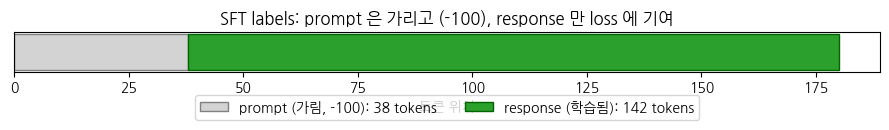
\includegraphics[width=0.86\linewidth]{assets/figures/ch28_sft_masking_bar.png}
\end{bookfigurelabel}

\textbf{그림 읽기} --- 그림~\ref{fig:ch28-sft-masking}에서 다음 내용을 확인합니다: SFT labels 마스킹: prompt는 제외하고 답변만 학습. 실행된 노트북에서 저장된 최신 plot 출력이므로, 코드에서 계산한 값이 어떤 평가 지점으로 이어지는지 바로 확인할 수 있습니다.



\section{\texorpdfstring{\inlinecode{SFTTrainer} 로 SFT 학습 --- \emph{새 trainer, 같은 loss 종류}}{SFTTrainer 로 SFT 학습 --- 새 trainer, 같은 loss 종류}}

\inlinecode{trl.SFTTrainer} 는 본 장에 처음 등장하는 클래스입니다. \inlinecode{transformers.Trainer} 를 상속해 \emph{SFT 에 특화된 전처리} (prompt/completion 토큰화, EOS 부착, completion 마스킹) 를 자동으로 해 줍니다. 설정은 \inlinecode{SFTConfig} (── \inlinecode{TrainingArguments} 를 상속) 로 주며, \textbf{\inlinecode{completion\_only\_loss=True}} 가 \emph{답변 부분만 학습} 하라는 핵심 옵션입니다.



\Needspace{11\baselineskip}
\begin{lstlisting}
from trl import SFTTrainer, SFTConfig

PROMPTS = [
    "피보나치 수열을 설명해줘",
    "건강한 식습관 3가지를 알려줘",
    "파이썬으로 리스트를 뒤집는 방법은?",
    "아침에 일찍 일어나는 팁을 알려줘",
]
GEN_KWARGS = dict(max_new_tokens=80, do_sample=True, temperature=0.8,
                  top_k=50, repetition_penalty=1.3)

\end{lstlisting}

\noindent\emph{앞 블록은 필요한 라이브러리와 기본 설정을 준비하는 단계입니다. 이어지는 블록에서는 텍스트를 모델 입력 텐서로 바꾸는 단계로 넘어갑니다.}

\Needspace{11\baselineskip}
\begin{lstlisting}[firstnumber=12]
@torch.no_grad()
def generate_answer(active_model, instruction: str, **kwargs):
    '''instruction 을 포맷해 답변을 생성. RESPONSE_TEMPLATE 뒤부터를 답변으로 디코드.'''
    text = build_prompt(instruction)
    enc = tokenizer(text, return_tensors="pt").to(active_model.device)
    out = active_model.generate(
        **enc,
        pad_token_id=tokenizer.pad_token_id,
        eos_token_id=tokenizer.eos_token_id,
        **kwargs,
    )
    full = tokenizer.decode(
        out[0],
        skip_special_tokens=True,
    )

\end{lstlisting}

\noindent\emph{앞 블록은 텍스트를 모델 입력 텐서로 바꾸는 단계입니다. 이어지는 블록에서는 앞에서 만든 중간 값을 다음 계산으로 넘기는 단계로 넘어갑니다.}

\Needspace{11\baselineskip}
\begin{lstlisting}[firstnumber=28]
    if RESPONSE_TEMPLATE.strip() in full:
        return full.split(RESPONSE_TEMPLATE.strip(), 1)[-1].strip()
    return full[len(text):].strip()

torch.manual_seed(SEED)
model.eval()
before_outputs = []
print("=" * 70)
print(
    "BEFORE SFT - raw KoGPT2 (no instruction tuning yet)"
)
print("=" * 70)
\end{lstlisting}

\noindent\emph{앞뒤 블록은 모두 앞에서 만든 중간 값을 다음 계산으로 넘기는 단계입니다. 길이를 나누어 같은 흐름을 단계별로 확인합니다.}

\Needspace{7\baselineskip}
\begin{lstlisting}[firstnumber=40]
for p in PROMPTS:
    ans = generate_answer(model, p, **GEN_KWARGS)
    before_outputs.append(ans)
    print(f"\n[instruction] {p}")
    print(f"[answer] {ans[:240]}")
\end{lstlisting}

\noindent\textbf{출력.}
\begin{bookoutputbox}
======================================================================
BEFORE SFT - raw KoGPT2 (no instruction tuning yet)
======================================================================

[instruction] 피보나치 수열을 설명해줘
[answer] 일단 한 번만 들어주면 끝나요
이제 본격적으로 사용하셔야겠죠?
다음부터는 내가 쓰는게 다인 듯!
내 안에 있는 피보라인의 모든 부분을 소개해드려요! momeljae.eats & pet_bang...
#미소천사 님이네요.
아무튼 저는 매일 미소에 대한

[instruction] 건강한 식습관 3가지를 알려줘
[answer] #diet #dieter #dietfood #eatclean <16.01.13.Sun>  
오늘은 정말 맛있는 날!
오랜만에 먹는 떡볶이가 나왔는데~ 진짜 너무 맛있었다
...
\end{bookoutputbox}
\par\vspace{0.9em}



\section{\texorpdfstring{학습 곡선 --- \emph{답변 부분에서만 계산된} loss}{학습 곡선 --- 답변 부분에서만 계산된 loss}}

아래 loss 는 \emph{답변 토큰에서만} 계산된 값입니다 (prompt 는 \inlinecode{-100} 으로 제외). \ref{ch:27}장의 loss (거의 모든 자리) 와는 \emph{합산 대상} 이 다르므로 절대값을 직접 비교하지는 않습니다.



\compactCodeOmitted{학습 설정을 만들고 학습 루프를 실행하는 단계}

\begin{bookfigurelabel}[H]{KoGPT2 SFT 학습 곡선과 VRAM 추적}{fig:ch28-sft-loss-vram}
\centering
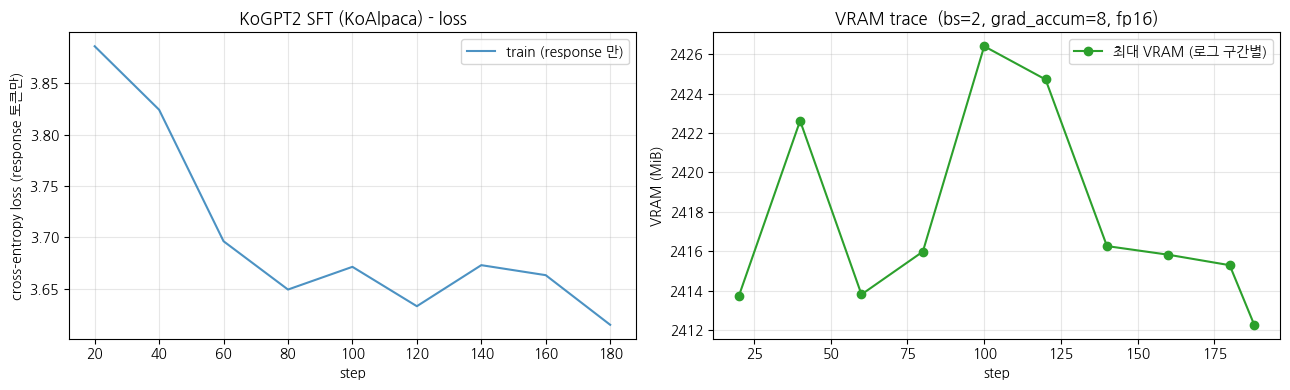
\includegraphics[width=0.88\linewidth]{assets/figures/ch28_sft_loss_vram_trace.png}
\end{bookfigurelabel}

\textbf{그림 읽기} --- 그림~\ref{fig:ch28-sft-loss-vram}에서 다음 내용을 확인합니다: KoGPT2 SFT 학습 곡선과 VRAM 추적. 실행된 노트북에서 저장된 최신 plot 출력이므로, 코드에서 계산한 값이 어떤 평가 지점으로 이어지는지 바로 확인할 수 있습니다.



\section{\texorpdfstring{SFT 전·후 instruction following 비교 --- \emph{행동 정렬이 일어났는가}}{SFT 전·후 instruction following 비교 --- 행동 정렬이 일어났는가}}

본 장의 핵심 데모. \emph{같은 instruction} 을 \emph{SFT 전 (raw KoGPT2)} 과 \emph{SFT 후} 에 각각 넣어 답변을 비교합니다.

\begin{itemize}
\tightlist
\item
  \textbf{SFT 전 (raw KoGPT2)}: instruction 을 \emph{지시로 인식하지 못하고} --- 질문을 \emph{이어쓰기} 하거나, 동화처럼 계속 쓰거나, 엉뚱한 방향으로 흐름
\item
  \textbf{SFT 후}: instruction 을 \emph{따라} --- 질문에 \emph{대답} 하는 구조화된 답변
\end{itemize}

이 차이가 \emph{행동 정렬 (behavior alignment)} 의 직접 증거입니다.



\textbf{해석 가이드 --- behavior alignment 의 증거}

\begin{itemize}
\tightlist
\item
  \textbf{BEFORE (raw KoGPT2)}: 같은 \emph{125M 본체} 인데도 instruction 을 \emph{지시로 받아들이지 못합니다}. \inlinecode{"피보나치\ 수열을\ 설명해줘"} 를 넣으면 \emph{설명} 대신 \emph{질문을 이어 쓰거나}, 일반 산문으로 흘러가거나, 동화체로 새는 경향
\item
  \textbf{AFTER (KoGPT2 + KoAlpaca SFT)}: \emph{같은 본체} 가 이제 instruction 을 \emph{따라} --- 질문에 \emph{대답하는} 구조로 응답. 짧은 SFT (1 epoch, 약 3K 샘플) 만으로도 \emph{행동의 방향} 이 바뀝니다
\end{itemize}

\begin{quote}
\textbf{핵심}: 본체는 \emph{한 토큰도 바꾸지 않은 같은 125M KoGPT2} 입니다 (continual pretraining 처럼 \emph{데이터만} 바뀐 게 아니라, \emph{데이터 형식 + 마스킹 자리} 가 바뀌었습니다). 그 결과 \emph{모델의 행동 자체} 가 instruction 을 따르도록 정렬됐습니다. \textbf{이게 \emph{왜 GPT 하나가 모든 task 를 해내는가} 의 답} --- 입력 프롬프트 형식만 바꾸면 다른 일을 하도록, SFT 가 그 능력을 \emph{깨웠습니다}.
\end{quote}

\begin{quote}
주의 KoGPT2 는 125M 의 \emph{작은} 모델이고 SFT 데이터·시간도 작아서, 답변 품질 자체는 거칠 수 있습니다 (사실 오류, 반복 등). 본 장의 관전 포인트는 \emph{답변의 정확도} 가 아니라 \emph{\textbf{instruction 을 따라가는 행동 자체가 생겼는가}} 입니다. 품질은 \emph{더 큰 모델 + 더 많은 데이터 + LoRA} 로 끌어올립니다 (FAQ 참고).
\end{quote}



\section{변형: 더 많은 데이터 / 다른 response\_template / LoRA}

본 장에서 다루지 못한 변형들 --- 직접 시도해 보고 싶다면 아래를 출발점으로:

\subsection{변형 1. 더 많은 데이터 / epoch}

\Needspace{5\baselineskip}
\begin{lstlisting}

\end{lstlisting}

\subsection{변형 2. 다른 response\_template}

\Needspace{5\baselineskip}
\begin{lstlisting}

\end{lstlisting}

\subsection{변형 3. LoRA / QLoRA --- 더 큰 모델 SFT}

\Needspace{9\baselineskip}
\begin{lstlisting}
# from peft import LoraConfig
# peft_config = LoraConfig(r=16, lora_alpha=32, 
# target_modules=["c_attn"],
# lora_dropout=0.05, task_type="CAUSAL_LM")
# trainer = SFTTrainer(model=model, args=sft_config, 
# train_dataset=sft_ds,
# processing_class=tokenizer, peft_config=peft_config)
\end{lstlisting}



\section{이 장에 등장한 라이브러리·함수}

\begin{booktable}{28장 새로 등장한 라이브러리}{tab:ch28-08}
\begin{adjustbox}{max width=\textwidth}
\begin{tabular}{@{}lll@{}}
\toprule
이름 & 한 줄 설명 & \ref{ch:27}장과 차이 \\
\midrule

\inlinecode{trl.SFTTrainer} & SFT 특화 trainer (prompt/completion 전처리 + completion 마스킹 자동) & \textbf{새로 등장} (\ref{ch:27}장 은 \inlinecode{transformers.Trainer}) \\
\inlinecode{trl.SFTConfig} & \inlinecode{SFTTrainer} 설정 (\inlinecode{TrainingArguments} 상속 + SFT 옵션) & \textbf{새로 등장} \\
\inlinecode{SFTConfig(completion\_only\_loss=True)} & \emph{답변 부분만} loss (prompt = \inlinecode{-100}) --- SFT 의 핵심 옵션 & \textbf{새로 등장} \\
\inlinecode{trl} 의 SFT collator (\inlinecode{DataCollatorForLanguageModeling}) & \inlinecode{completion\_mask} 로 prompt 를 \inlinecode{-100} 마스킹 & \textbf{새로 등장} (\ref{ch:27}장 은 \inlinecode{transformers.DataCollatorForLanguageModeling(mlm=False)}) \\
\inlinecode{prompt} / \inlinecode{completion} 데이터 형식 & instruction-response 쌍 표준 형식 & \textbf{새로 등장} (\ref{ch:27}장 은 단일 \inlinecode{text} 컬럼) \\
\inlinecode{AutoModelForCausalLM.from\_pretrained("skt/kogpt2-base-v2")} & KoGPT2 본체 로드 & \textbf{공유} (\ref{ch:27}장과 같은 본체) \\
\inlinecode{PreTrainedTokenizerFast.from\_pretrained("skt/kogpt2-base-v2",\ ...)} & KoGPT2 BBPE 토크나이저 (AutoTokenizer 함정 회피) & \textbf{공유} (\ref{ch:27}장과 동일) \\
\inlinecode{model.generate(repetition\_penalty=...)} & 반복 억제 sampling (작은 모델의 반복 완화) & \textbf{약간 다름} (반복 페널티 추가) \\
\bottomrule
\end{tabular}
\end{adjustbox}
\end{booktable}

\begin{quote}
\inlinecode{trl} 은 버전마다 API 변동이 큰 라이브러리입니다 (\inlinecode{DataCollatorForCompletionOnlyLM} 처럼 버전에 따라 사라진 클래스도 있습니다). 본 노트북은 \emph{\inlinecode{prompt}/\inlinecode{completion} 데이터 + \inlinecode{completion\_only\_loss=True}} 라는 \emph{최신 trl 의 표준 경로} 를 씁니다 --- 이 경로가 버전 간 가장 안정적입니다. 설치된 \inlinecode{trl} 버전은 셋업 셀의 출력에서 확인하세요.
\end{quote}



\section{체크포인트 질문}

\begin{enumerate}
\def\labelenumi{\arabic{enumi}.}
\tightlist
\item
  SFT 에서 \emph{왜 prompt 부분을 \inlinecode{-100} 으로 가리나요?} 만약 prompt 도 학습 대상에 포함하면 (response-only 가 아니라 전체 학습) 모델은 무엇을 강화하게 되고, 왜 그게 instruction following 에 불리한가요?
\item
  \emph{Continual pretraining (\ref{ch:27}장)} 과 \emph{SFT (\ref{ch:28}장)} 는 \emph{같은 본체 + 같은 next-token CrossEntropyLoss} 를 씁니다. 그런데도 둘은 다른 단계입니다 --- 정확히 \emph{무엇 두 가지} 가 다른가요? (데이터 형식 / \inlinecode{labels\ =\ -100} 자리)
\item
  \texttt{\#\#\#\ 응답:\textbackslash{}n} (response\_template) 의 역할은 무엇인가요? collator 는 이 문자열을 어떻게 사용해 prompt 와 답변을 나누나요?
\item
  \emph{“같은 모델이 입력 프롬프트만 바꾸면 다른 task 를 한다”} --- BERT 단계 (task 마다 새 head) 와 비교해 이게 왜 가능한가요? SFT 가 그 능력에서 하는 역할은?
\end{enumerate}



\section{FAQ}

\begin{faqBox}{Q1. (이론) SFT 가 continual pretraining (\ref{ch:27}장) 과 정확히 뭐가 다른가요?}

\emph{같은 본체, 같은 next-token \inlinecode{CrossEntropyLoss}} 를 쓴다는 점은 같습니다. 다른 건 \textbf{두 가지}:

\begin{booktable}{28장 FAQ 표}{tab:ch28-09}
\begin{adjustbox}{max width=\textwidth}
\begin{tabular}{@{}lll@{}}
\toprule
항목 & Continual pretraining (\ref{ch:27}장) & SFT (\ref{ch:28}장) \\
\midrule

\textbf{데이터 형식} & 연속된 일반 텍스트 (TinyStories) & \textbf{instruction-response 쌍} (KoAlpaca) \\
\textbf{\inlinecode{labels\ =\ -100} 자리} & pad 만 (거의 모든 자리 학습) & \textbf{prompt 부분 전체} (답변만 학습) \\
\bottomrule
\end{tabular}
\end{adjustbox}
\end{booktable}

\Needspace{5\baselineskip}
\begin{lstlisting}
SFTConfig(completion_only_loss=True)
\end{lstlisting}

continual pretraining 은 \emph{모델의 지식·도메인} 을 다듬고, SFT 는 \emph{모델의 행동 (지시를 따르는 법)} 을 정렬합니다. 그래서 실무에서는 보통 \emph{pretraining \(\to\) (continual pretraining) \(\to\) SFT \(\to\) alignment} 순서로 \emph{쌓아} 갑니다.

\end{faqBox}

\begin{faqBox}{Q2. (이론) 왜 prompt 를 \inlinecode{-100} 으로 가리나요? 가리지 않으면 어떻게 되나요?}

\emph{질문을 외우는 것} 과 \emph{답하는 법을 배우는 것} 의 차이입니다. prompt 도 학습 대상에 넣으면:

\begin{enumerate}
\def\labelenumi{\arabic{enumi}.}
\tightlist
\item
  loss 의 \emph{상당 부분} 이 \emph{prompt 토큰} 에서 나옵니다 (prompt 가 보통 답변보다 길거나 비슷). 모델은 \emph{질문을 받아쓰는} 데 gradient 를 씁니다
\item
  모델이 \emph{주어진 질문 분포} 에 과적합 --- \emph{새로운 질문} 에 약해질 수 있습니다
\item
  우리가 원하는 \emph{“질문이 주어졌을 때 답하는 능력”} (조건부 생성) 이 희석됩니다
\end{enumerate}

\texttt{labels{[}:prompt\_len{]}\ =\ -100} 한 줄로 \emph{prompt 는 조건 (given), 답변만 학습 대상 (target)} 으로 분리합니다. §3 에서 본 collator 출력이 정확히 이 효과입니다.

\Needspace{6\baselineskip}
\begin{lstlisting}
input_ids = tokenizer(prompt + response)["input_ids"]
labels = input_ids.copy()
prompt_len = len(tokenizer(prompt)["input_ids"])
labels[:prompt_len] = [-100] * prompt_len
\end{lstlisting}

\end{faqBox}

\begin{faqBox}{Q3. (실무) \inlinecode{SFTTrainer} 는 \inlinecode{transformers.Trainer} 와 뭐가 다른가요?}

\inlinecode{SFTTrainer} 는 \inlinecode{transformers.Trainer} 를 \emph{상속} 한 서브클래스입니다 --- 학습 루프 (forward / backward / optimizer step) 는 \emph{완전히 동일}. 다른 건 \emph{데이터 전처리를 자동화} 한다는 점:

\begin{itemize}
\tightlist
\item
  \emph{prompt + completion} 을 토큰화해 이어 붙이고, 답변 끝에 \textbf{EOS 를 자동 부착}
\item
  \inlinecode{completion\_only\_loss=True} 면 \emph{completion 마스킹} (\inlinecode{completion\_mask} 생성 \(\to\) prompt \inlinecode{-100}) 을 자동
\item
  (옵션) \inlinecode{packing}, chat template 적용 등 SFT 편의 기능
\end{itemize}

\Needspace{5\baselineskip}
\begin{lstlisting}
trainer = SFTTrainer(model=model, args=SFTConfig(completion_only_loss=True),
                     train_dataset=sft_ds, processing_class=tokenizer)
\end{lstlisting}

즉 \emph{같은 학습 루프, 더 적은 보일러플레이트}. SFT 의 \emph{마스킹 같은 디테일} 을 라이브러리가 처리해 줍니다.

\end{faqBox}

\begin{faqBox}{Q4. (이론) chat template 이 뭔가요? KoGPT2 는 왜 직접 포맷하나요?}

\textbf{chat template} 은 \emph{대화 메시지 (\texttt{\{“role”:\ “user”,\ “content”:\ ...\}}) 를 모델이 학습한 형식의 문자열로 변환하는 규칙} 입니다. instruction-tuned 모델 (예: Llama-Instruct, Qwen-Chat) 은 토크나이저에 chat template 이 내장돼 있어 \inlinecode{tokenizer.apply\_chat\_template(messages)} 한 줄로 포맷됩니다.

\textbf{KoGPT2 는 \emph{base 모델} (instruction tuning 안 됨) 이라 chat template 이 없습니다.} 그래서 우리가 \emph{직접} 포맷합니다:

\Needspace{5\baselineskip}
\begin{lstlisting}
def build_prompt(instruction):
    return f"### 명령어:\n{instruction}\n\n### 응답:\n"
\end{lstlisting}

\begin{quote}
\emph{우리가 정한 포맷} (\inlinecode{\#\#\#\ 명령어:} / \inlinecode{\#\#\#\ 응답:}) 으로 SFT 하면, \emph{추론 시에도 같은 포맷} 으로 입력해야 합니다. SFT 가 \emph{그 포맷을 모델의 chat template 으로} 가르치는 셈입니다. instruction-tuned 모델을 \emph{직접 만드는} 과정이 곧 \emph{그 모델의 chat template 을 정의} 하는 일입니다.
\end{quote}

\end{faqBox}

\begin{faqBox}{Q5. (실무) 더 큰 모델을 SFT 하려면? LoRA / QLoRA 는 무엇인가요?}

KoGPT2 (125M) 는 T4 에서 full fine-tuning 이 가능하지만, \emph{7B 급 이상} 은 full SFT 가 \emph{T4 메모리 (16GB) 를 초과} 합니다. 그래서 실무 표준은 \textbf{LoRA} (Low-Rank Adaptation):

\begin{itemize}
\tightlist
\item
  본체 weight 는 \emph{freeze} (그대로 두고)
\item
  각 layer 에 \emph{작은 low-rank adapter 행렬 (\inlinecode{r=8-64})} 만 추가해 \emph{그것만 학습}
\item
  학습 파라미터가 \emph{전체의 약 0.1-1\%} \(\to\) 메모리·시간 대폭 절감
\end{itemize}

\textbf{QLoRA} 는 여기에 \emph{본체를 4bit 양자화} 까지 더해 \emph{더 큰 모델 (예: 70B) 도 단일 GPU} 에서 SFT 가능하게 합니다.

\Needspace{7\baselineskip}
\begin{lstlisting}
from peft import LoraConfig
peft_config = LoraConfig(r=16, lora_alpha=32, target_modules=["c_attn"],
                         lora_dropout=0.05, task_type="CAUSAL_LM")
trainer = SFTTrainer(model=model, args=sft_config, train_dataset=sft_ds,
                     processing_class=tokenizer, peft_config=peft_config)
\end{lstlisting}

본 장은 \emph{full SFT} (LoRA 없이) 로 \emph{마스킹의 원리} 에 집중했습니다. LoRA 는 \emph{메모리 기법} 일 뿐 \emph{마스킹·loss 원리는 동일} 합니다.

\end{faqBox}

\begin{faqBox}{Q6. (실무) SFT 후 답변 품질이 거친데요? (반복, 사실 오류)}

KoGPT2 는 \emph{125M 의 작은 base 모델} 이고, 본 장의 SFT 는 \emph{약 3K 샘플 / 1 epoch} 로 \emph{최소 규모} 입니다. 그래서:

\begin{itemize}
\tightlist
\item
  \textbf{반복} --- \inlinecode{model.generate(repetition\_penalty=1.3)}, \inlinecode{no\_repeat\_ngram\_size=3} 등으로 완화
\item
  \textbf{사실 오류 / 환각} --- 작은 모델의 근본 한계. 더 큰 모델 + RAG (검색 증강) 로 보완
\item
  \textbf{포맷 일관성} --- 더 많은 데이터 / epoch 로 개선
\end{itemize}

\begin{quote}
본 장의 목표는 \emph{답변의 정확도} 가 아니라 \emph{\textbf{instruction 을 따라가는 행동 자체가 생겼는가}} 입니다. §6 의 BEFORE/AFTER 에서 \emph{지시를 따르는 방향} 으로 바뀌었다면 SFT 의 핵심 (행동 정렬) 은 성공한 것입니다. 품질은 \emph{모델 크기 + 데이터 + LoRA} 의 영역.
\end{quote}

\end{faqBox}

\begin{faqBox}{Q7. (이론) 다음 단계 alignment (DPO, \ref{ch:30}장) 는 SFT 와 뭐가 다른가요?}

SFT 는 \emph{“좋은 답변 하나” 를 따라 학습} 합니다 (정답 demonstration 모방). 하지만 \emph{“여러 답변 중 어느 게 더 나은가”} 라는 \emph{선호 (preference)} 는 가르치지 못합니다. \textbf{alignment (DPO 등)} 가 그 단계:

\begin{booktable}{28장 FAQ 표}{tab:ch28-10}
\begin{adjustbox}{max width=\textwidth}
\begin{tabular}{@{}lll@{}}
\toprule
단계 & 데이터 & 학습 신호 \\
\midrule

\textbf{SFT (\ref{ch:28}장)} & instruction \(\to\) \emph{하나의} 좋은 답변 & 그 답변을 \emph{따라 생성} \\
\textbf{DPO (\ref{ch:30}장)} & instruction \(\to\) \emph{(chosen, rejected) 쌍} & chosen 을 \emph{더 선호}, rejected 를 \emph{덜 선호} \\
\bottomrule
\end{tabular}
\end{adjustbox}
\end{booktable}

\begin{quote}
흥미롭게도 DPO 도 \emph{\inlinecode{labels\ =\ -100} thread 를 잇습니다} --- chosen / rejected 각각의 \emph{response 부분에서만} log-likelihood 를 계산합니다 (prompt 는 양쪽 공통이라 제외). 즉 \emph{답변 부분만 본다} 는 본 장의 원리가 alignment 까지 이어집니다. DPO 는 \ref{ch:30}장에서 본격.
\end{quote}

\Needspace{5\baselineskip}
\begin{lstlisting}
# from trl import DPOTrainer, DPOConfig
\end{lstlisting}
\end{faqBox}



\begin{previewBox}{미리보기: 다음 장}

\textbf{\ref{ch:29}장. 벤치마크 평가 --- SFT 모델을 분야별 벤치마크로 측정}

\begin{itemize}
\tightlist
\item
  본 장에서 만든 \emph{SFT 모델} 을 \emph{정량 벤치마크} 로 평가: 한국어 (KMMLU / HAERAE-Bench / LogicKor / KoBEST) + 영어 (MMLU / HellaSwag / GSM8K ...)
\item
  \inlinecode{lm-evaluation-harness} 로 \emph{task-format 별} 자동 평가 --- \emph{instruction following 이 점수로 드러나는가}
\item
  \emph{SFT 전 (base) vs SFT 후} 벤치마크 비교 --- §6 의 정성적 BEFORE/AFTER 를 \emph{정량} 으로
\item
  그 다음 \ref{ch:30}장 (DPO) --- \emph{preference 정렬}. \textbf{\inlinecode{labels\ =\ -100} thread 가 DPO 에서도 이어집니다} --- chosen/rejected \emph{response 부분만} 계산
\end{itemize}

\textbf{Phase 4 GPT 시대 4단계 흐름 정리}:

\begin{booktable}{28장 FAQ 표}{tab:ch28-11}
\begin{adjustbox}{max width=\textwidth}
\begin{tabular}{@{}lllll@{}}
\toprule
장 & 단계 & 본체 & 데이터 & \inlinecode{labels\ =\ -100} 자리 \\
\midrule

\ref{ch:24}·\ref{ch:26}장 & 1 (pretraining) & 작은 GPT scratch & TinyStories (영/한) & pad 만 \\
\ref{ch:25}·\ref{ch:27}장 & 2 (continual pretraining) & gpt2 / KoGPT2 & TinyStories (동일) & pad 만 \\
\textbf{\ref{ch:28}장 \(\leftarrow\) 여기} & \textbf{3 (SFT)} & \textbf{KoGPT2 (동일)} & \textbf{KoAlpaca instruction-response} & \textbf{prompt 부분 (답변만 학습)} \\
\ref{ch:30}·\ref{ch:31}장 & 4 (alignment) & SFT 모델 + ref & preference / verifier reward & response 부분만 (RL 내부) \\
\bottomrule
\end{tabular}
\end{adjustbox}
\end{booktable}

\begin{quote}
\textbf{변하는 축} (\ref{ch:27}장 \(\to\) \ref{ch:28}장): \emph{학습 단계} (continual pretraining \(\to\) SFT). 본체·토크나이저·loss 종류는 같고, \emph{데이터 형식 + \inlinecode{labels\ =\ -100} 자리} 가 바뀝니다. 본 장에서 그 \emph{마스킹 자리} 를 collator 출력으로 \emph{눈으로 확인} 했습니다 --- 그게 Phase 4 두 thread 의 클라이맥스입니다.
\end{quote}
\end{previewBox}